

We now explain our support for local transactions with SI semantics in the
context of a system as described in Section~\ref{sec:context} above. We first define the API and
semantics of local transactions (Section~\ref{ssec:lc-api}) and then continue to describe our
solution, which consists of two parts. First, in Section~\ref{ssec:region-clock}, we enhance the
underlying data store with support for per-region local version clocks and an
API to manipulate this clock jointly with objects stored at that region. This
entails a minor modification to management of global timestamps (in the TM or oracle). 
Second, we add client-side support for local transactions, as explained in Section~\ref{ssec:lc-client}.

\subsection{Local transactions: API and semantics} \label{ssec:lc-api}

We support a restricted set of local transactions, focusing on short ones that
frequently occur in production. Recall that short transactions benefit most from
our optimizations since for them, the overhead of performing centralized coordination once or twice
per transaction is significant.

There are two distinctive characteristics of local transactions. First, they
must access a single region. Second, in contrast to regular transactions, they
cannot dynamically evolve, but rather must be provided in their entirety with a
single API call: 
local transactions forgo the standard API including begin and commit operations,
and instead invoke a single function for executing the entire transaction. The
new API functions for local transactions are prefixed with \code{LTX\_}. 

The simplest examples are singleton transactions, i.e., transactions that perform a single
read operation via \code{LTX\_read(key)} or a single update via \code{LTX\_write(key, value)}. 
The latter creates a new version for key that exceeds all existing ones.

A more elaborate example is a multi-read-single-write API, \code{LTX\_MRSW(\wkey, \rkeys, f)}, 
which atomically reads values associated  with a list of \rkeys and updates the value associated with
\wkey according to some function f of the read values. Note that this API
is applicable only in case \wkey and all \rkeys reside in the same region. In case
they do not, the call fails, and the transaction may be restarted as a regular
transaction.

The semantics for ordering local transactions relative to regular ones are
weaker than SI in that they do not guarantee real-time order over all regular
and local transactions together. Specifically, a regular transaction overlapping
two local transactions that access different regions may observe the updates of
the second and miss an update by the first. For example, assume objects x and y
are managed in two different regions, then real-time order can be violated as
illustrated in Figure~\ref{fig:ltx-rt} (ignore the skip operations for now; they will be explained in the next section).

\begin{figure}[h]
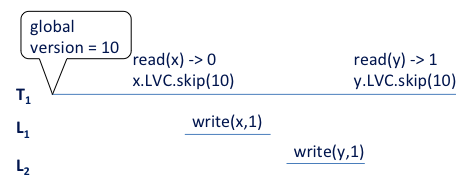
\includegraphics[width=\columnwidth]{LTX-RT}
\caption{Possible violation of real-time order among local transactions in different regions. Global transaction $T_1$
reads $x$ before it is updated by local transaction $L_1$ and reads $y$ after it is updated by local transaction $L_2$ even 
though $L_2$ occurs after $L_1$. $T1$'s global version is $10$, and its skips the local version clocks of the regions holding $x$ and $y$ to $10$ when reading from them.}
\label{fig:ltx-rt}
\end{figure}

The system still enforces a total order on all committed transactions, so that
\begin{enumerate}
    \setlength{\itemsep}{0pt}
    \setlength{\parskip}{0pt}
    \setlength{\parsep}{2pt}  
\item
regular transactions (though not local ones) are ordered according to their commit times;
\item
each transaction's read operations see a consistent snapshot of the database reflecting 
a sequence of transactions that includes all those committed prior to
its start time plus any number of concurrent local transactions; and 
\item
 a transaction commits only if none of the items it updates has been modified since that snapshot.
 \end{enumerate}

\idit{Todo: add a note about causality being preserved because re-ordering can only occur across regions.}

\subsection{Data store and timestamp management extensions} \label{ssec:region-clock}

We add some functionality to a region, to be used exclusively by our client-side
extensions given in Section 3.3 below. The key mechanism used to support local
transactions is a local version clock (LVC) per region. Like the GVC, LVCs are
also monotonically increasing. Each region has its
own LVC. In Section~\ref{ssec:lvc} we describe this local clock's API and its impact on
the GVC. We then proceed to present the extension of the data store API for
accessing objects together with the LVC in Section~\ref{ssec:lvc-access}.

\subsubsection{Local version clock} \label{ssec:lvc}

\idit{Todo: generalize the discussion in this subsection to encompass CockroachDB, which does not have a GVC, and whose local clocks are essentially updated similarly to our LVC to reflect causality relations.}

Each region's LVC is loosely synchronized with the GVC. The idea is to use the
region's LVC for ordering local transactions in any given region, and allow
local transactions to progress in different regions independently. Note that it
is safe to do so because no global order needs to be enforced among transactions
that access disjoint sets of objects.

Multi-region transactions, in turn, continue to obtain their versions from the
GVC. Therefore, whenever a multi-region transaction $T$ accesses a given region,
we have to synchronize that region's LVC with the GVC in order to ensure that
the version obtained by $T$ exceeds those obtained by earlier completed
transactions within the region, and that later transactions within that region
will obtain higher versions than $T$'s.

To support such loose synchronization, the GVC now advances at a coarse
granularity of epochs. This can be implemented, for example, by choosing some
epoch size $2^\ell$, and keeping the $\ell$ least significant bits of the GVC padded
with zeros. In other words, every increment of the GVC increases its value by
$2^\ell$.
The LVC obtains the epoch ($n-\ell$ most-significant bits for an $n$-bit GVC) from the
GVC, and proceeds to assign timestamps within the designated epoch (by
incrementing the least significant bits).

The LVC has a single component, LVC.current, and it supports the following API:
\begin{description}
\item[\code{LVC.skip(epoch)}] -- atomically set LVC.current to max(epoch, LVC.current) .

\item[\code{LVC.fetchAndIncrement()}] -- atomically increment LVC.current and return new
value.
For simplicity, we assume that the LVC is used so it does not overrun the epoch
and does not wrap around within the epoch. That is, fetchAndIncrement is called
less than $2^\ell$ times in each epoch.

\item[\code{LVC.get()}] -- return LVC.current.
\end{description}

By incrementing the GVC, a multi-region transaction essentially initiates a new
epoch, and obtains a timestamp exceeding all those of older local transactions.
In addition, multi-region transactions enforce the synchronization of the LVC
with respect to the GVC using the skip operation. Specifically, whenever a
transaction in a new epoch accesses (for either read or write intention
indication) an object in a region whose LVC is still in an older epoch, it
invokes that region's LVC.skip so it will not lag behind the transaction's
read-timestamp obtained from the GVC. Thus, new local transactions that will
begin later in the region will have higher timestamps, as needed.

Note that transaction commits do not alter the LVC; the LVC only reflects
transactions' read-timestamps obtained when they  begin.

Note also that as long as a running transaction does not access a given region,
further updates can occur by local transactions in that region, and these
updates can be reflected in the transaction's snapshot in case it later reads
these objects. Thus, unlike with regular transactions, which satisfy real-time
order, a transaction's snapshot may reflect changes that occur after it
commences, as in the example of Figure~\ref{fig:ltx-rt}.

Here, x is written with LVC=10 and later y is written with its LVC=0. The
concurrent transaction's snapshot time is 10, which includes the update of x and
not that of y. The same scenario does not occur with two local transactions
accessing the same region, since once the LVC is incremented, not further
updates in the same region can occur with older LVC values.



\subsubsection{Accessing data and the LVC together} \label{ssec:lvc-access}

In order to allow local transactions to execute with a single data store access,
we extend the data store to support functions that access data objects and the
LVC together. Thus, a local transaction can increment LVC, obtain a version, and
write with this version, all in one round-trip to the local data store.

We further enforce atomic access to the data and the LVC. This is important in
order to avoid races between obtaining a version from the LVC and updating the
data. For example, if the updates of the LVC and the data were separate, the
following scenario could have arisen:
\begin{itemize}
  \item Local transaction $L_1$ plans to update object A and obtains LVC value 2.
  \item Multi-region transaction $T_1$ obtains read version 2.
  \item Local transaction $L_2$ obtains LVC value 3 and updates object B.
  \item Multi-region transaction $T_2$ obtains read version 3.
  \item $T_2$ reads the old version of A (since it had not been written by $L_1$ yet)
  and the new version of  B.
  \item $L_1$ writes A with 2 and completes.
  \item $T_2$ reads the new version of A and the old version of  B.
\end{itemize}
Here, SI is violated.

In addition, the new functions must take care not to breach the  atomicity of
concurrent transactions. To this end, they rely on the write intention indications.
We extend the data store with the following functions, whose 
pseudocode is given in Algorithm~\ref{alg:lvc-and-data}. 

\begin{description}
  \item[\code{mutate(key, value)}] atomically increments the region's LVC
  and creates a new version for key associated with the new LVC value. The
  operation fails (returns false) if the latest version of the object has a write intention
  indication. 
  \item [\code{validateAndMutate(\wkey, \wversion, value, robjs)}]
 where \robjs = $\langle$ \rkey, \rversion $\rangle$*  is an optional parameter.
Atomically validates that the provided versions of \wkey and \rkeys (if
applicable)  are equal to the highest ones in the data store and mutates the
object associated with \wkey and the LVC as mutate does. Returns true if the
validation is successful, otherwise returns false and does not perform the
mutation. 
Note that the version numbers provided with the object parameters correspond to
old versions; they are used for validation, and are not stored with the new
version. The new version is produced using the LVC.
\item [\code{collect(keys)}]   
returns a consistent snapshot of version-value pairs pertaining to keys. 
In particular, it selects a $ts$, which is the region's LVC at some point during its execution, and returns the version with the highest version that does not have a write intention indication associated with each key up to this $ts$. 
\end{description}

\begin{algorithm}[htb]
\begin{algorithmic}
\Procedure{mutate}{key, value} 
\If{ \code{hasWriteIntent(key)} }
return false
\EndIf
\State  version $\leftarrow$ \code{LVC.fetchAndIncrement()}
\State add $\langle$ version, value $\rangle$ to key
\State return true
\EndProcedure
\Statex
%
\Procedure{validateAndMutate}{\wkey, \wversion, value, $\langle$ \rkey, \rversion $\rangle$*}
\If{ \code{hasWriteIntent(key)}}
	\State return false
\EndIf
\If{latest version of \wkey $\neq$  \wversion}
	\State return false
\EndIf
\ForAll{\rkey,\rversion}
 	\If{latest version of \rkey $\neq$ \rversion} 
    		\State return false
    	\EndIf
 \EndFor
\State  version $\leftarrow$ \code{LVC.fetchAndIncrement()}
\State add $\langle$ version, value $\rangle$ to key
\State return true
\EndProcedure
\Statex
%
\Procedure{collect}{keys}
\State $ts \leftarrow$ \code{LVC.get()}
\ForAll{key $\in$ keys} 
	\State S $\leftarrow \{ \langle$
	% \rangle \}$ 
	key, version, value $\rangle$ in data store $|$ 
\State	$\neg$ \code{hasWriteIntent(key, version, value)} $\wedge$ 
\State version $\leq ts \}$ 
	\State add argmax$_S$ (version) to snapshot
 \EndFor
\State return $\langle$ snapshot, $ts \rangle$
\EndProcedure

\end{algorithmic}
\caption{Methods for atomic access of LVC and data in a single region. Each method executes atomically.}
\label{alg:lvc-and-data}
\end{algorithm}


\subsection{Client-side support for local transactions} \label{ssec:lc-client}

Pseudocode for the client-side implementation of various local transaction types is given in 
Algorithm~\ref{alg:ltx-client}. 
Singletons are implemented directly using the new functions in the underlying data store.
The next type of local transaction is a single-key read-and-write,  \code{LTX\_SRW}. It is
parametrized by some compute function f that generates the new value from the old one.
Because \code{LTX\_SRW} does not perform the update to the data store atomically
with the read, it needs to validate the mutate operation to ensure that the object
has not been updated since its latest version was read at the beginning of the
operation. If the validation fails, the transaction can be retried, either the
same way or using a regular transaction.
Finally, we extend this operation to read from multiple objects and update one, 
using \code{LTX\_MRSW}.

\begin{algorithm}[htb]
\begin{algorithmic}
\Procedure{LTX\_read}{key} 
\State  return collect(key).array
\EndProcedure
 % 
\Procedure{LTX\_write}{key, value} 
\State  return mutate(key, value)
\EndProcedure
%
\Procedure{LTX\_SRW}{key, f} 
\State $\langle$ version, value $\rangle \leftarrow$ read(key)
\State  return \code{validateAndMutate(key, version, f(value))}
\EndProcedure
%
\Procedure{LTX\_MRSW}{\wkey, \rkeys, f} 
\State \Comment \rkeys is a non-empty list 
\State $\langle$ snap, ts $\rangle \leftarrow$ \code{collect(keys)}
 \State return \code{validateAndMutate(\wkey, ts, f(snap), snap)}
\EndProcedure
\end{algorithmic}
\caption{Client-side code for local transactions.}
\label{alg:ltx-client}
\end{algorithm}

